\documentclass{elsart}
%\usepackage{fullpage}

%\usepackage{graphicx}
\usepackage{amsmath}
\usepackage{latexsym}
\usepackage{theorem}
\usepackage{amssymb}
\usepackage{amsfonts}
\usepackage{url}
\usepackage{graphicx}
\journal{CGTA}

\newcommand{\patscomment}[1]{}

%%% \setlength{\parindent}{0mm}
%%% \setlength{\parskip}{2mm}
%\setlength{\parskip}{1ex}

%%%%%%%%%%%%%%% FOR THE BEAUTIFUL IPE PICTURES  %%%%%%%%%%%%%%%%%%%%%%%
%\def\Ipe#1{\def\IPEfile{#1}\input{#1}}

%%%%%%%%%%%%%%%%%%%%%  SOME ABBREVIATIONS %%%%%%%%%%%%%%%%%%%%%%%%%%%%%%
\newcommand{\Nats}{{\mathbb{N}}}             % natural numbers
\newcommand{\Reals}{{\mathbb{R}}}            % real numbers
\newcommand{\Euclid}{{\mathbb{E}}}           % Euclidean space
\newcommand{\eps}{\varepsilon}               % epsilon
\newcommand{\obj}{{\mathcal C}}                  % object
\newcommand{\scene}{{\mathcal S}}                % scene
\newcommand{\bd}{\partial}                   % boundary
\newcommand{\dir}{\vec{d}}                   % direction
\newcommand{\dist}{\mathrm{dist}}            % distance

\newcommand{\defsym}{:=}                     % for definitions
\newcommand{\Mid}{:}                         % used in {p \Mid p \in BLA}

\newcommand{\ranges}{{\mathcal R}}
\newcommand{\meas}[1]{\mu(#1)}
\newcommand{\pmeas}[1]{\mu_P(#1)}
\newcommand{\qmeas}[1]{\mu_Q(#1)}

\newcommand{\card}[1]{\mbox{card}(#1)}

\newcommand{\discrepancy}{\Delta}
\newcommand{\dis}{\discrepancy}
\newcommand{\pqdis}[1]{\discrepancy_{P,Q}(#1)}
\newcommand{\rdis}[1]{\discrepancy_{\ranges}(#1)}
\newcommand{\pdis}[1]{\discrepancy_{P}(#1)}

\newcommand{\disH}{\discrepancy_{\HH}(S)}
\newcommand{\disF}{\discrepancy_{\FF}(S)}

\newcommand{\signeddiscrepancy}{\delta}
\newcommand{\sdis}[1]{\signeddiscrepancy(#1)}
\newcommand{\sdisc}[1]{\overline{\signeddiscrepancy}(#1)}

\newcommand{\error}[1]{\Delta(#1)}
\newcommand{\areadiscrepancy}{\Delta^*}
\newcommand{\adis}[1]{\areadiscrepancy(#1)}

\newcommand{\radius}[1]{\mathrm{radius}(#1)} % radius
\newcommand{\diam}[1]{\mathrm{diam}(#1)}     % diameter
\newcommand{\area}[1]{\mathrm{area}(#1)}     % area
\newcommand{\rank}{\mathrm{rank}}     % rank
\newcommand{\vol}[1]{\mathrm{vol}(#1)}       % volume
\newcommand{\mylength}[1]{\mathrm{length}(#1)} % length
\newcommand{\peri}[1]{\mathrm{peri}(#1)}     % perimeter
\newcommand{\refp}[1]{\mathrm{ref}(#1)}      % reference point
\newcommand{\ch}[1]{\mathrm{CH}(#1)}         % convex hull
\newcommand{\bb}{\mathrm{bb}}                % bounding box
\newcommand{\fat}[1]{\mathrm{fatness}(#1)}   % fatness

\newcommand{\A}{{\mathcal A}}
\newcommand{\B}{{\mathcal B}}
\newcommand{\D}{{\mathcal D}}
\newcommand{\disc}{{\mathcal D}}
\newcommand{\HH}{{\mathcal H}}
\newcommand{\LL}{{\mathcal L}}
\newcommand{\V}{{\mathcal V}}
\newcommand{\tree}{{\mathcal T}}

\newcommand{\node}{\nu}
\newcommand{\pa}[1]{\mathrm{pa}(#1)}
\newcommand{\err}[1]{\mbox{err}(#1)}
\newcommand{\serr}[1]{\mbox{S-err}(#1)}
\newcommand{\lerr}[1]{\mbox{L-err}(#1)}
\newcommand{\verr}[1]{\mbox{V-err}(#1)}
\newcommand{\add}[1]{\mathrm{add}(#1)}
\newcommand{\mypos}{\mathrm{pos}}
\newcommand{\myneg}{\mathrm{neg}}

\newcommand{\cell}{C}
\newcommand{\face}{F}

%%%%%%% make "less (greater) than or equal to" look nice
%\let\leq\leqslant %% DOESN'T WORK FOR SOME REASON
%\let\geq\geqslant

%%%%%%%%%%%%%%%%%%%%% DEFS FOR THEOREMS AND SUCH %%%%%%%%%%%%%%%%%%%%%%%
%
% All of these are used as follows:
%     \begin{environmentname}  ..... \end{environmentname}
% where "environmentname" is the unabbreviated version of what
% you want (theorem, lemma, etc.)
%
%%%%%%%%%%%%%%%%%%%%%%%%%%%%%%%%%%%%%%%%%%%%%%%%%%%%%%%%%%%%%%%%%%%%%%%%
%\theorembodyfont{\normalfont\slshape}
%\theorempreskipamount \theorempostskipamount

\newtheorem{definition}{Definition}[section]
\newtheorem{theorem}[definition]{Theorem}
\newtheorem{lemma}[definition]{Lemma}
\newtheorem{corollary}[definition]{Corollary}
\newtheorem{observation}[definition]{Observation}
\newtheorem{remark}[definition]{Remark}

\newenvironment{proof}{{\bf Proof:} \rm}{\hfill $\Box$ \medskip\\}

%%%%%%%%%%%%%%%%%%%%%%  FOR COMMENTS %%%%%%%%%%%%%%%%%%%%%%%%%%%%%%%%%%%%%
%\newcommand{\comment}[1]{\begin{quotation} {\footnotesize *** #1 *** } \end{quotation}}

%
% Formatting different from standard
%
%\makeatletter
%\partopsep\z@ \textfloatsep 10pt plus 1pt minus 4pt
%\def\section{\@startsection {section}{1}{\z@}{-3.5ex plus -1ex minus
%-.2ex}{2.3ex plus .2ex}{\large\bf}}
%\def\subsection{\@startsection{subsection}{2}{\z@}{-3.25ex plus -1ex
%minus -.2ex}{1.5ex plus .2ex}{\normalsize\bf}}
%\def\@fnsymbol#1{\ensuremath{\ifcase#1\or \ast\or {\ast}\!{\ast}\or
%    {\ast}\!{\ast}\!{\ast}\else\@ctrerr\fi}} 
%\makeatother



\begin{document}
\begin{frontmatter}
\title{On Simplifying Dot Maps\thanksref{nserc}}
\thanks[nserc]{This research was partly supported by NSERC.}

\author[eindhoven]{Mark de Berg}, 
\author[carleton]{Prosenjit Bose}, 
\author[eindhoven]{Otfried Cheong}, and 
\author[carleton]{Pat Morin}

\address[eindhoven]{Department of Computer Science, TU Eindhoven, PO
Box 513, 5300 MB Eindhoven, the Netherlands}
\address[carleton]{School of Computer Science,
          Carleton University, 
          1125 Colonel By Drive, Ottawa, Ontario, Canada
          K1S 5B6}.
	  
%%%%%%%%%%%%%%%%%%%%%%%%%%%%%%%%%%%%%%%%%%%%%%%%%%%%%%%%%%%%%%%%%%%
\begin{abstract}
  Dot maps---drawings of point sets---are a well known cartographic method
  to visualize density functions over an area. We study the problem of
  simplifying a given dot map: given a set $P$ of points in the plane,
  we want to compute a smaller set~$Q$ of points whose distribution
  approximates the distribution of the original set~$P$.

  We formalize this using the concept of $\eps$-approximations, and we
  give efficient algorithms for computing the approximation error of a set $Q$
  of $m$ points with respect to a set $P$ of $n$ points (with $m \leq n$)
  for certain families of ranges, namely unit squares,
  arbitrary squares, and arbitrary rectangles.

  If the family $\ranges$ of ranges is the family of all possible unit
  squares, then we compute the approximation error of $Q$ with respect
  to $P$ in $O(n\log n)$ time. If $\ranges$ is the family of all
  possible rectangles, we present an $O(mn\log n)$ time algorithm.  If
  $\ranges$ is the family of all possible squares, then we present a
  simple $O(m^2n + n \log n)$ algorithm and an $O(n^2\sqrt{n}\log n)$
  time algorithm which is more efficient in the worst case.

  Finally, we develop heuristics to compute
  good approximations, and we evaluate our heuristics experimentally.
\end{abstract}

\begin{keyword}
Dotmaps \sep discrepancy \sep $\eps$-approximations
\end{keyword}
\end{frontmatter}

%%%%%%%%%%%%%%%%%%%%%%%%%%%%%%%%%%%%%%%%%%%%%%%%%%%%%%%%%%%%%%%%%%%

%%%%%%%%%%%%%%%%%%%%%%%%%%%%%%%%%%%%%%%%%%%%%%%%%%%%%%%%%%%%%%%%%%%
\section{Introduction}\label{se:intro}
%%%%%%%%%%%%%%%%%%%%%%%%%%%%%%%%%%%%%%%%%%%%%%%%%%%%%%%%%%%%%%%%%%%
%\paragraph{Background.}
%%%%%%%%%%%%%%%%%%%%%%%%%%%%%%%%%%%%%%%%%%%%%%%%%%%%%%%%%%%%%%%%%%%
An important component in the area of cartography is the ability to
represent and visualize the distribution or density of some phenomenon
such as the population distribution over a certain region. The most
common technique to achieve this is the \emph{dot map}, as shown in
Fig.~\ref{fi:dotmap}.  The term \emph{dot map} is
self-explanatory---it refers to the use of dots or points placed on a
map to represent a given distribution. Dot maps are quite important
and their use has been extensively studied in cartography---see for
instance Chapter 8 of the book by Dent~\cite{d-ctmd-99}.
%%%%%%%%%%%%%%%%%%%%%%%%%%%%%%%%%%%%%%%%%%%%%%%%%%%%%%%%%%%%%%%%%
\begin{figure}[htb]
\begin{center}
  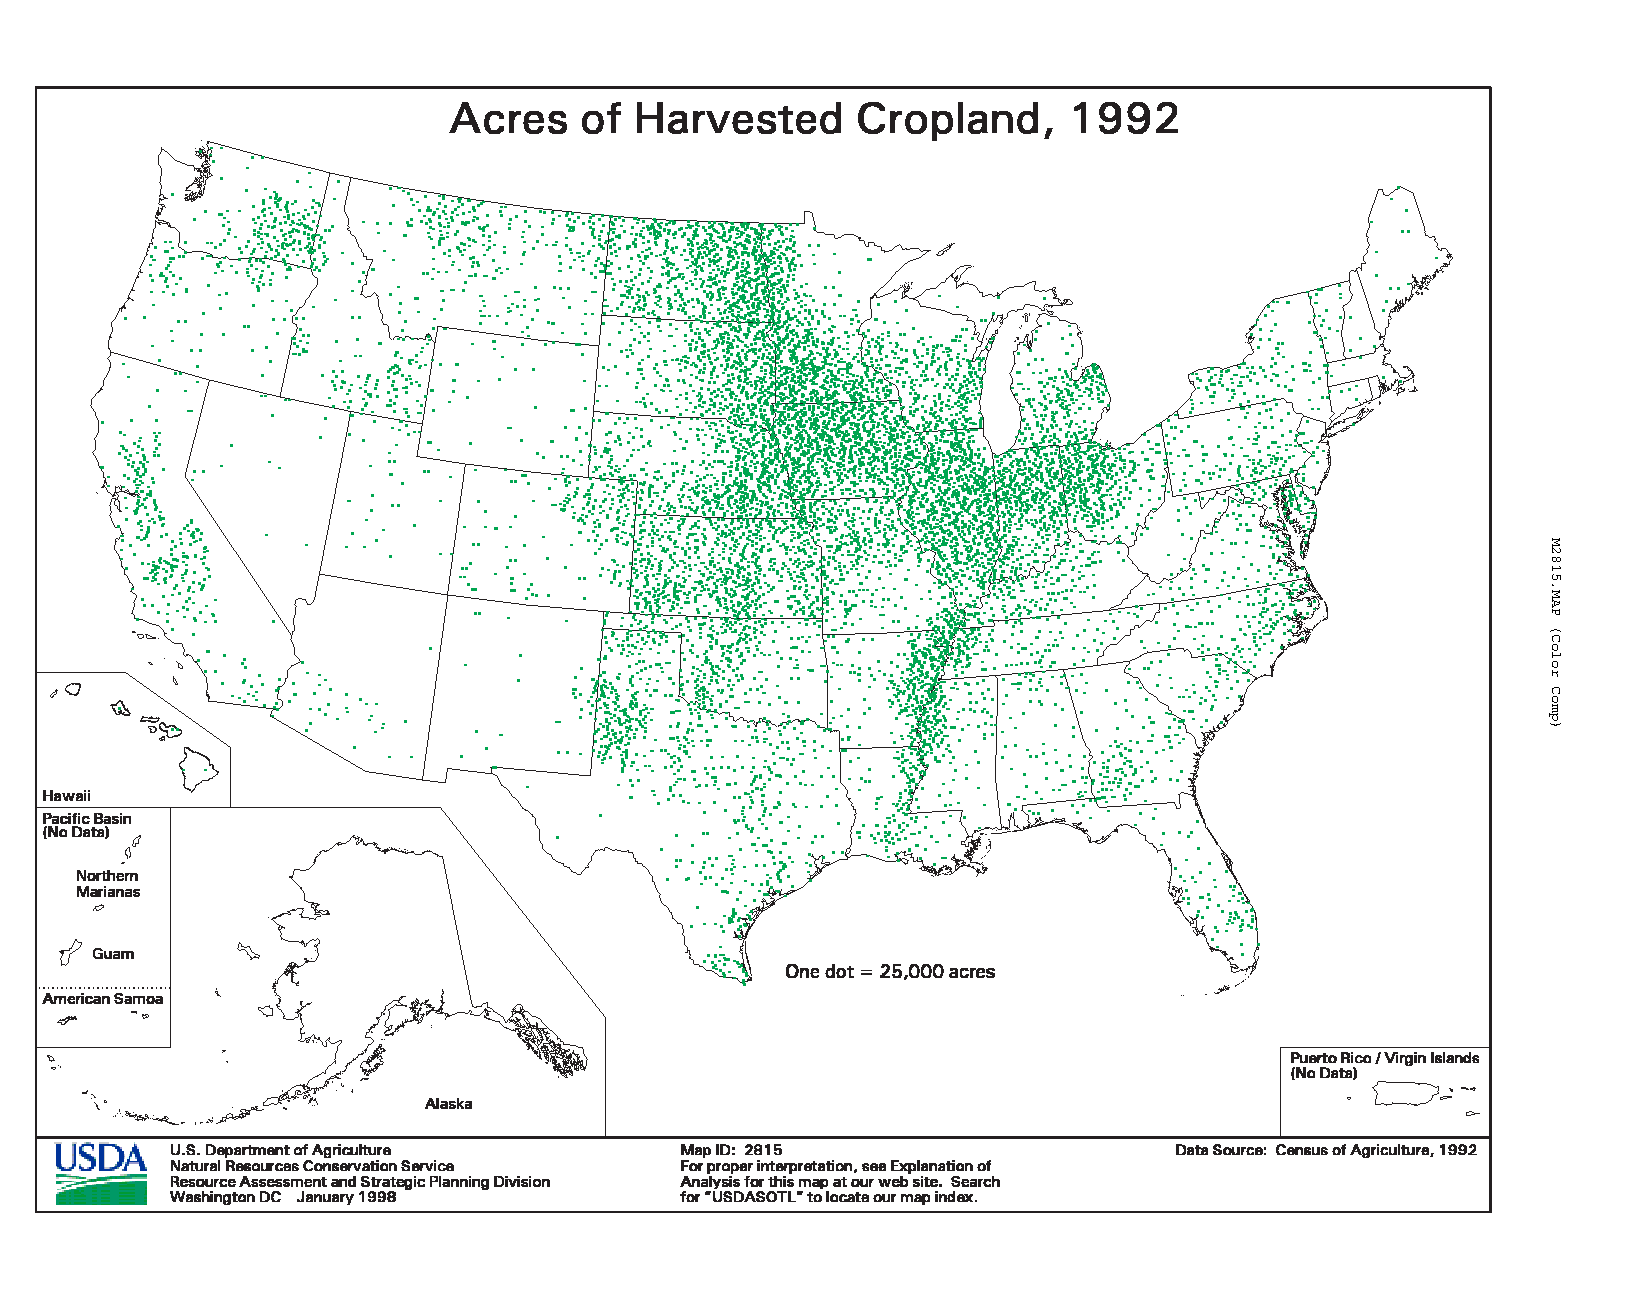
\includegraphics[scale=0.5]{m2815}
\end{center}
\caption{Example of a dot map.}
\label{fi:dotmap}
\end{figure}
%%%%%%%%%%%%%%%%%%%%%%%%%%%%%%%%%%%%%%%%%%%%%%%%%%%%%%%%%%%%%%%%%

There are many issues involved in the use of dot maps as a tool for
representing distributions. For example, the radius of the dots used, or
the decision to allow or disallow dots to overlap are important visual
considerations~\cite{d-ctmd-99}. Depending on the application, it can
also be important to take the topographic `background map' into account:
a dot map representing population density should not have dots
inside lakes, in mountainous areas one may have to take altitude into
account, and it may be important to ensure that dots are
on the correct side of borders or other features~\cite{ditz}.
In this paper, we concentrate on two related computational issues
that purely deal with distribution issues; visual considerations
and adherence to a background map are beyond the scope of this paper.

The first question we study is: Given a point
set $P$ representing a certain distribution, how can we automatically
simplify it, that is, generate a smaller representative point set $Q$
of a given size?  This question arises when one wishes to scale a map:
the number of points in the map has to decrease when the size of the map
is decreased, otherwise it would become too cluttered. It may also arise
in the generation of the initial dot map: ``The printed dot map
of the population distribution should be constructed at a larger scale
based on more detailed information such as settlements and houses
and then reduced to the final scale.'', as Ditz~\cite{ditz} writes.
The first question---how can we compute a
good approximation?---immediately leads to the second: Given sets $P$
and $Q$, how can we determine the quality of $Q$ as an approximation
to $P$?
%%%%  Both these questions have already been addressed in the GIS
%%%%  and cartographic communities~\cite{d-ctmd-99}.  WHERE?
%%%%  Add ref to Monika if we have it !!
To determine the quality of an approximation, we need a
quantatitive measure of similarity between dot maps.
Our measure is inspired by interactive GISs
where a user can use a dot map of, say, the population
density, to estimate the population within a region~\cite{ditz}.
This can either be a user-defined area---a square, for example---or a
geographically meaningful region such as the area within a certain
distance from a river. This leads us to propose the notion of
$\eps$-approximations~\cite{vc71} as a quantitative measure
of the quality of an approximation.
A set $Q$ of $m$ points is called an \emph{$\eps$-approximation} of
a set $P$ of $n$ points\footnote{Traditionally, in the definition of
$\eps$-approximation it is required that $Q\subset P$, but this is not
necessary.} with respect to a family $\ranges$ of ranges, if for any
range $r \in \ranges$ we have
\[
\left| \;\; |r \cap P|/n - |r \cap Q|/m \;\; \right| \leq \eps.
\]
In other words, if we approximate the number of points from $P$ inside a
range $r$ by multiplying the number of points from $Q$ inside the range by
$n/m$, then we make an error of at most $\eps n$.
This leads us to define $\Delta_{\ranges}(Q,P)$, the \emph{approximation
error of $Q$ with respect to $P$}, for a family $\ranges$ of ranges, as
\[
\Delta_{\ranges}(Q,P)
   = \max_{r\in\ranges} | |r \cap P| - (n/m) \cdot |r \cap Q| |.
\]
The value $n/m$, which can be viewed as the weight of a point in $Q$
as compared to a point in $P$, is called the \emph{dot value} of the points in $Q$.
We usually denote it by $\delta$.
In this paper we focus on squares and rectangles\footnote{In this
paper squares and rectangles are always axis-parallel.}  as ranges.
Of these types of ranges, squares are probably most natural in our
application. Another natural range to consider would be discs.

%%%%%%%%%%%%%%%%%%%%%%%%%%%%%%%%%%%%%%%%%%%%%%%%%%%%%%%%%%%%%%%%%%%
\subsection{Related work.}
%%%%%%%%%%%%%%%%%%%%%%%%%%%%%%%%%%%%%%%%%%%%%%%%%%%%%%%%%%%%%%%%%%%
$\eps$-Approximations have been studied and used extensively in
computational geometry---see for instance Chazelle's
book~\cite{c01}---and various algorithms are known to compute
$\eps$-approximations of asymptotically optimal size for a set $P$ and
a given value of~$\eps$. Note that we want to solve a slightly
different problem: in our case $\eps$ is not given, but the desired
number of points in the approximation~$Q$. Still, one may use the same
type of algorithms. For instance, in many cases it turns out that
random sampling is expected to produce an approximation of
asymptotically optimal size. (One caveat is in place here: the
optimality here refers to the worst-case size of an
$\eps$-approximation over all point sets $P$ of $n$ points, not to the
minimum size needed for the given set $P$. These two sizes need not be
the same.) Thus, for our problem we could simply take a random subset
$Q\subset P$ of the desired size. Then, of course, one would want
to check how good the sample is, that is, one needs an algorithm
to compute the approximation error of given sets $P$ and $Q$.

The use of $\eps$-approximations to measure the similarity of two
point sets is related to some statistical methods to derive a
(continuous) density function from a given point set; see the book by
Baily and Gatrell~\cite{bg-isda-95} for more information on
statistical methods for spatial data analysis.  For example, kernel
estimation defines the density $\lambda(x)$ at a point $x$ in the
plane by summing the number of points within a region around the point
$x$ in a weighted manner; the shape of the region and the exact
weighting scheme depends on the kernel used.  Comparing two point
sets---for example, to see whether the distribution of some feature of
the population (number of cancer deaths, for instance) deviates from
the population distribution itself---is then done by comparing the
density functions $\lambda_1(x)$ and $\lambda_2(x)$ obtained for the
two points sets. Usually one takes the quotient of these two values,
but if one wants to bound the worst-case error this doesn't work
($\lambda_2(x)$ may be zero) and one could take the absolute
difference.  The notion of $\eps$-approximation with unit squares as
ranges can be seen as a special case of this, where the kernel is a
block function with value~1 inside the unit square centered at the
point $x$ and value~0 elsewhere (and the other parameters of the
kernel estimation method choosen suitably).  The advantage of such a
simple kernel function is that it is computationally easier, in the
sense that it makes computing the approximation error easier.  Recall
that the motivation behind our use of $\eps$-approximations is that we
want to bound the maximum error when an approximating set $Q$ is used
to estimate the number of points from a set $P$ inside a range. The
size of such a range is not fixed in an interactive setting. Hence, we
also look at squares of arbitary sizes, which makes our error measure
different from traditional kernel methods.

The approximation error as defined above is a generalization of the
\emph{bichromatic discrepancy} (or \emph{combinatorial discrepancy}).
Here one colors each point of a given set either red or blue and one
is interested in the maximum difference, over all possible ranges of
the given family, between the number of red points and the number of
blue points inside a range.  If we call the red point set $P$ and the
blue point set $Q$, and we define the dot value to be~1 (even when
$|P| \neq |Q|$), then the bichromatic discrepancy equals the
approximation error.  Also, finding an optimal red-blue coloring of a
given set~$P$ is identical to finding a subset $Q \subset P$ such that
the discrepancy of $Q$ with respect to $P$ and dot value~2 is
minimized.  The concept of bichromatic discrepancy arises in
computational learning theory, in particular in the so-called
minimizing disagreement problem in agnostic
PAC-learning~\cite{dg95,gk00}.  Thus our algorithms to compute the
approximation error of two given sets with respect to a family
$\ranges$ of ranges may be used to solve the minimizing disagreement
problem when the class of hypotheses is $\ranges$---see the paper by
Dobkin~et~al.~\cite{dgm96} for details.

Finally, we note that our problem is related to that of computing the
\emph{area discrepancy} (or \emph{continuous discrepancy}) of a point
set~$P$. This is a measure of how uniform that point set is, and it
has applications in computer graphics~\cite{dgm96,dem96,s-dqmsd-91}.

%%%%  \comment{I omitted refs to book by Devroye and Lugosi (don't know
%%%%    what's in there) and to Ostromoukov (read it, but does not
%%%%    seem directly related) and Ulichney (don't know what's in there).
%%%%    We should remove thse refs from the Refs unless we cite them after all.
%%%%  
%%%%    Also, we do not cite Monika Sester, and the ref to Ditz has no
%%%%    proceedings name etc.}

%%%%%%%%%%%%%%%%%%%%%%%%%%%%%%%%%%%%%%%%%%%%%%%%%%%%%%%%%%%%%%%%%%%
\subsection{Our results.}
%%%%%%%%%%%%%%%%%%%%%%%%%%%%%%%%%%%%%%%%%%%%%%%%%%%%%%%%%%%%%%%%%%%
Computing the approximation error of a set $Q$ of $m$ points with respect
to a set $P$ of $n$ points, with $m\leq n$,
is the topic of Section~\ref{se:theory}. We obtain the following results.
If $\ranges$ is the family of all possible unit squares, then we can
compute the approximation error of $Q$ with respect to $P$ in $O(n\log n)$
time. If $\ranges$
is the family of all possible rectangles, then we present two algorithms,
a simple $O(m^2n + n \log n)$ algorithm and a more efficient $O(mn\log
n)$ time algorithm.  This is a slight improvement over an algorithm
of Dobkin~et~al.~\cite{dgm96} when $m$ is $o(n)$. Their algorithm runs
in $O(n^2\log n)$ time regardless of how small $m$ is.  If $\ranges$ is
the family of all possible squares, then we present a simple $O(m^2n +
n \log n)$ algorithm and an $O(n^2\sqrt{n}\log n)$ time algorithm which
is more efficient in the worst case.

We turn our attention in Section~\ref{se:experiments} to
the experimental component of the paper. The goal is to develop
heuristics to generate for a given set $P$ an approximation $Q$ of the
desired size with as small an error as possible.  We concentrate on
the case of square ranges, as this seems most relevant to our
application.
Our heuristics use as a subroutine an algorithm to compute the error
for given $P$ and $Q$. Unfortunately, our algorithm for arbitrary
squares is rather slow, and some of the heuristics call this
subroutine many times.  Hence, we first show experimentally that the
exact error with respect to squares can be approximated well by
computing the error with respect to fixed-size squares for a number of
different sizes.  After having established this, we compare
various heuristics to find a good approximation of a given
point set~$P$. One of our findings is that taking the best
approximation out of a large collection of random samples does
not work so well, even though random sampling is guaranteed
to find approximations that are asymptotically worst-case optimal.

%%%%%%%%%%%%%%%%%%%%%%%%%%%%%%%%%%%%%%%%%%%%%%%%%%%%%%%%%%%%%%%%%%%
\section{Computing the approximation error}
\label{se:theory}
%%%%%%%%%%%%%%%%%%%%%%%%%%%%%%%%%%%%%%%%%%%%%%%%%%%%%%%%%%%%%%%%%%%
Let $P$ be a set of $n$ points and $Q$ be a set of $m$ points in the
plane, with $m\leq n$. In this section we show how to compute the
approximation error of $Q$ with respect to $P$ for three different
families of ranges: unit squares, arbitrarily sized squares, and
arbitrarily sized rectangles. By $\delta\defsym n/m$ we denote the dot
value of the points in~$Q$.

%%%%%%%%%%%%%%%%%%%%%%%%%%%%%%%%%%%%%%%%%%%%%%%%%%%%%%%%%%%%%%%%%%%
\subsection{Unit squares as ranges}
\label{subse:unitsquares}
%%%%%%%%%%%%%%%%%%%%%%%%%%%%%%%%%%%%%%%%%%%%%%%%%%%%%%%%%%%%%%%%%%%
Let $\ranges$ be the family of all possible unit squares.  When we
want to compute the approximation error of $Q$ with respect to $P$ for
unit squares, it can make a difference whether we consider open or
closed squares. In the description of the algorithm, we will consider
the squares to be closed; it is easy to adapt the algorithm to the
case of open squares.

Recall that we use the absolute value of the error in the definition
of approximation error.  It is convenient to compute separately the
maximum positive error and the maximum negative error. Below we
describe how to compute the maximum positive error; computing the
maximum negative error can be done in a similar way.

A unit square contains a point if and only if the center of the unit
square is contained in the unit square centered at the point. Hence,
instead of considering the point sets $P$ and $Q$ and the family of
all unit squares as ranges, we can use the sets $S_P$ and $S_Q$ of
unit squares centered at the points in $P$ and $Q$, and all points in
the plane as ranges. Call the squares in $S_P$ the \emph{red squares},
and the squares in $S_Q$ the \emph{blue squares}. The (positive)
approximation error of a point $x$ in the plane is now
\[
\mbox{(\# of red squares containing $x$)} -
  \delta \cdot \mbox{(\# of blue squares containing $x$)}.
\]
The approximation error of $S_Q$ with respect to $S_P$ is the maximum
approximation error over all points in the plane. From the
discussion above it follows that this is the same as the approximation
error of $Q$ with respect to $P$ for the family $\ranges$ of unit
squares as ranges.

The arrangement formed by the squares $S_Q$ and $S_P$ partitions the
plane into faces where the approximation error of any point in a face
of the arrangement is the same. Therefore, finding the maximum
approximation error amounts to finding the face with maximum
approximation error. We compute the approximation of $S_Q$ with
respect to $S_P$ with a plane-sweep algorithm. In this algorithm, we
sweep a vertical line $\ell$ from left to right over the
arrangement. As we sweep the arrangement, we maintain the maximum
approximation error over the faces of the arrangement intersected by
$\ell$. Since the arrangement is formed by squares, the only events
are when the sweep lines reaches a left or right edge of a square. At
each event we compute the maximum error of all points on $\ell$ and of
all points slightly to the right of $\ell$ (but to the left of the
previous event). The maximum error found in all the events will be the
maximum error of $S_Q$ with respect to $S_P$.
We now describe the
information we maintain during the sweep---the status structure---and
how to handle the events.

%%%%%%%%%%%%%%%%%%%%%%%%%%%%%%%%%%%%%%%%%%%%%%%%%%%%%%%%%%%%%%%%%%%
\subsubsection{A dynamic 1-dimensional structure.}
%%%%%%%%%%%%%%%%%%%%%%%%%%%%%%%%%%%%%%%%%%%%%%%%%%%%%%%%%%%%%%%%%%%
The status structure is a dynamic data structure for solving the
following 1-dimensional version of the problem. We are given a set
$I_R$ of red segments and a set $I_B$ of blue segments on the real line,
and a parameter $\delta$. The (positive) approximation error
of a point~$x\in \Reals$ is defined as
\[
\mbox{(\# of red segments containing~$x$)} -
\delta \cdot \mbox{(\# of blue segments containing~$x$)}.
\]
We want to maintain the maximum error over
all points in $\Reals$  under insertions and deletions of segments.

The structure we use is essentially the structure described in
\cite{bkmmm-trgps-01} in the context of grid placement problems.
A similar structure is also presented in \cite{dgm96}. 
The structure maintains a function $f:\Reals \to \Reals$. Initially, it is
assumed that $f(x) = 0$, for all $x \in \Reals$. The following update
and query operations are allowed on the structure:

\begin{enumerate}
\item Insert($[a:b], d$): Increase the value of $f(x)$ by $d$ over the interval
$[a:b]$.
\item Delete($[a:b], d$): Decrease the value of $f(x)$ by $d$ over the interval
$[a:b]$.
\item Max(): Return $\max\{f(x):x \in \Reals\}$.
\end{enumerate}

The first two operations can be performed in $O(\log n)$ time where
$n$ is the number of intervals currently inserted and the third
operation takes $O(1)$ time.
  Essentially, the data structure is a
  balanced binary tree (similar to a segment tree~\cite{bkos-cgaa-97}) whose
  leaves represent the \emph{elementary intervals} (of the inserted
  intervals) ordered from left to right. An internal node of the tree
  represents the interval that is the union of the elementary intervals
  of the leaves in its subtree.  The nodes have been augmented with
  additional information in order to answer the queries. The structure
  has $O(n)$ size where $n$ is the number of intervals currently in the
  structure. For more details on the structure, the reader is referred
  to the paper of Bose et al.~\cite{bkmmm-trgps-01}.

With this structure, the 1-dimensional problem is easily solved. When
inserting (resp.  deleting) a red segment, we increase
(resp. decrease) the value of $f(x)$ by 1 over this
segment. Similarly, when inserting (resp. deleting) a blue segment, we
decrease (resp. increase) the value of $f(x)$ by $\delta$ over this
segment. Max() allows one to recover the maximum
approximation error over the currently inserted segments.


This leads to the following lemma.
%%%%%%%%%%%%%%%%%%%%%%%%%%%%%%%%%%%%%%%%%%%%%%%%%%%%%%%%%%%%%%%%%%%
\begin{lemma}\label{le:1d_dynamic}
The maximum approximation error of a set of red and blue segments on a
line can be maintained with a structure of $O(n)$ space that takes
$O(\log n)$ time per insertion and deletion, where $n$ is the number
of red and blue segments.
\end{lemma}
%%%%%%%%%%%%%%%%%%%%%%%%%%%%%%%%%%%%%%%%%%%%%%%%%%%%%%%%%%%%%%%%%%%

We now return to the 2-dimensional problem, where we want to compute
the approximation error of a set of blue squares with respect to a set
of red squares, with the points in the plane as ranges. Recall that
our approach is a plane-sweep algorithm. The algorithm maintains the
maximum error along the sweep line $\ell$ using the structure $\tree$
just described above. Whenever the left edge of a square is
encountered, we insert its $y$-interval into the structure along with
the appropriate value (that is, 1~if it is red and $-\delta$ otherwise),
and whenever the right edge of a square is encountered, we delete its
$y$-interval. If events happen simultaneously---multiple edges have
the same $x$-coordinate---then we process the events in the following
order. First we handle all left boundaries. After this, Max() tells
us the maximum error on $\ell$. Next, we handle all the right
boundaries, and get the maximum error slightly to the right of
$\ell$. Hence, every event takes $O(\log n)$ time to process and the
initialization takes $O(n\log n)$ time. Since there are $O(n)$ events
to process, we get the following theorem.
%%%%%%%%%%%%%%%%%%%%%%%%%%%%%%%%%%%%%%%%%%%%%%%%%%%%%%%%%%%%%%%%%%%
\begin{theorem}\label{th:unitsquares}
  Let $P$ be a set of $n$ points in the plane, and let $Q$ be a set of
  $m$ points in the plane, with $m \leq n$.  The approximation error
  of $Q$ with respect to $P$ for the family of all unit squares can be
  computed in $O(n\log n)$ time.
\end{theorem}

%%% \comment{Should we mention that given any convex distance function, this approach
%%% implies an $O(n^2)$ time algorithm since we can sweep the arrangement but now have to
%%% stop at every intersection point as well as every vertex.}
%%%%%%%%%%%%%%%%%%%%%%%%%%%%%%%%%%%%%%%%%%%%%%%%%%%%%%%%%%%%%%%%%%%


%%%%%%%%%%%%%%%%%%%%%%%%%%%%%%%%%%%%%%%%%%%%%%%%%%%%%%%%%%%%%%%%%%%
\subsection{Arbitrarily sized squares as ranges}
\label{subse:squares}
%%%%%%%%%%%%%%%%%%%%%%%%%%%%%%%%%%%%%%%%%%%%%%%%%%%%%%%%%%%%%%%%%%%
The case of squares of arbitrary size as ranges is probably the most
interesting in our application.
Note that, unlike in the case of unit squares, the approximation error does not
depend on whether we consider open or closed squares: for any open (closed)
square, there is a slightly smaller closed (larger open) square
that contains exactly the same points.
We start by showing a fairly simple
algorithm that runs in $O(m^2n +n\log n)$ time.

We first prove a lemma which restricts the number of candidate
squares. Let $B$ be the bounding box of $P\cup Q$.
%%%%%%%%%%%%%%%%%%%%%%%%%%%%%%%%%%%%%%%%%%%%%%%%%%%%%%%%%%%%%%%%%%%
\begin{lemma}\label{le:squares}
There is an open square with maximum positive error such that two
opposite sides of the square each either contain a point from $Q$ or
are contained in the boundary of $B$.
Similarly, there is a closed square with maximum negative error such that two
opposite sides of the square each contain a point from $Q$.
\end{lemma}
%%%%%%%%%%%%%%%%%%%%%%%%%%%%%%%%%%%%%%%%%%%%%%%%%%%%%%%%%%%%%%%%%%%
\begin{proof}
Let $s$ be an open square of maximum positive error, that is, a square
that maximizes $|r \cap P| - \delta \cdot |r \cap Q|$. Suppose the top
and right edge do not contain a point from $Q$ or a part of the boundary of
$B$. Fix the bottom left corner of $s$ and grow the square until
either a point from $Q$ or the boundary of $B$ hits the top or right
edge of $s$. No point of $P$ can enter $s$ during this process since
otherwise $s$ was not a maximum. Next, fix the top right corner of $s$
and grow the square until either a point from $Q$ or the boundary of
$B$ hits the bottom or left edge of $s$. Again, no point of $P$ can
enter $s$ during this process. At this point, the conditions of the
lemma are met or two adjacent edges of $s$ contain a point from $Q$ or
the boundary of $B$. If the latter holds, then assume, without loss of
generality, that the top and left edges of $s$ contain a point of
$Q$. Then fix the top left corner and grow the square until the
condition of the lemma is met.

Now let $s$ be a closed square of maximum negative error, and suppose
the top and right edge do not contain a point from $Q$ or a part of
the boundary of $B$. We can transform $s$ into a square with the same
error that satisfies the conditions of the lemma using the same
procedure as above, except this time we shrink $s$ instead of growing
$s$. Because of the shrinking, we do not have the case where the
boundary of $s$ hits the boundary of $B$, since we can assume that
initially $s$ lies completely inside $B$.  
\end{proof}

%%%%%%%%%%%%%%%%%%%%%%%%%%%%%%%%%%%%%%%%%%%%%%%%%%%%%%%%%%%%%%%%%%%

 %%%%%%%%%%%%%%%%%%%%%%%%%%%%%%%%%%%%%%%%%%%%%%%%%%%%%%%%%%%%%%%%%%%%%
 \subsubsection{A simple algorithm}
 %%%%%%%%%%%%%%%%%%%%%%%%%%%%%%%%%%%%%%%%%%%%%%%%%%%%%%%%%%%%%%%%%%%%%
Next we describe a simple algorithm, based on Lemma \ref{le:squares},
to compute the maximum positive approximation error;
the maximum negative error can be computed in a similar way.

 By Lemma \ref{le:squares},
 the square of maximum discrepancy must have
 a blue point (i.e. a point from $Q$) on two opposite sides. Given two
 blue points, if the absolute value of the difference in their
 $x$-coordinate is larger than the absolute value of the $y$-coordinate
 difference, then the two points can only lie on the left and right
 sides of a square. Similarly, if the $y$-coordinate difference is
 larger, than the two points can only lie on the top and bottom edges
 of the square. Finally, if the differences are the same, then there
 is a unique square with the points at the opposite
 corners. This implies that a given pair of blue points determines the
 size of the square and the direction of search. Since there are $m$
 blue points, there are $m \choose 2$ candidate pairs. Select one such
 pair, $q_i, q_j$, and assume without loss of generality that the
 $y$-coordinate difference is larger. The case where the $x$-coordinate
 difference is larger is symmetric, and the other case is trivial.


 Given $q_i$ and $q_j$, let $h_i$ and $h_j$ be the horizontal lines
 through the respective points.
 We have to find the maximum error over all squares whose top
 end bottom edges are contained in those lines.
 In order to find this maximum, we
 will sweep (i.e.~move) the square from left to right through the strip.

 Consider the points in $P\cup Q$ that lie within this strip. Sort
 these points by their $x$-coordinates, and let $S$ represent this set
 in sorted order. Start with the left boundary of the square on the
 left boundary of $B$. Compute the discrepancy of this square by
 finding the points of $S$ in this square. Now, sweep the square from
 left to right until the right boundary reaches the right boundary of
 $B$ and maintain the maximum at each step. The events in this sweep
 are that either a point leaves the square or a point enters the
 square. The order in which the points enter as well as the order in
 which the points leave is the sorted order. Processing an event
 amounts to adding or subtracting the appropriate amount to the current
 discrepancy, depending on which point enters or leaves. (Events that
 occur simultaneously should be handled together; the details of how
 this should be done are easy to fill in.)
 Note that we
 do not need to sweep the whole strip but only the portion of the strip
 where $q_i$ and $q_j$ are on the top and bottom edges of the
 square. However, this optimization does not make a difference
 asymptotically.  Since each event can be processed in $O(1)$ time
 given the sorted order, we can compute in $O(n)$ time the maximum
 discrepancy given a candidate pair of points provided the points in
 the strip are sorted. If we pre-sort the points of $P \cup Q$ in $O(n
 \log n)$ time then $O(n)$ time the sorted order of points of $P \cup
 Q$ within a strip can be obtained. Since there are $O(m^2)$ possible
 candidates and each candidate can be verified in $O(n)$ time, the
 total time for the algorithm is $O(m^2n + n\log n)$.

%%%%%%%%%%%%%%%%%%%%%%%%%%%%%%%%%%%%%%%%%%%%%%%%%%%%%%%%%%%%%%%%%%%%%
\begin{theorem}\label{th:sq_simple}
Let $P$ be a set of $n$ points in the plane, and let $Q$ be a set of
$m$ points in the plane, with $m \leq n$. The approximation error of
$P$ with respect to $Q$ for squares can be computed in $O(m^2n + n\log
n)$ time.
\end{theorem}
%%%%%%%%%%%%%%%%%%%%%%%%%%%%%%%%%%%%%%%%%%%%%%%%%%%%%%%%%%%%%%%%%%%%%

 %%%%%%%%%%%%%%%%%%%%%%%%%%%%%%%%%%%%%%%%%%%%%%%%%%%%%%%%%%%%%%%%%%%%%
  \subsubsection{A subcubic algorithm}
 %%%%%%%%%%%%%%%%%%%%%%%%%%%%%%%%%%%%%%%%%%%%%%%%%%%%%%%%%%%%%%%%%%%%%
The algorithm of Theorem~\ref{th:sq_simple} runs in cubic time if $m=\Theta(n)$.
Next we describe a subcubic algorithm.
Recall that in the case of unit squares as ranges, we replaced every
point in $P\cup Q$ with a unit square and we looked at the maximum
error of points in the plane with respect to the resulting sets $S_P$
and $S_Q$ of squares. This approach does not apply here since the size
of the square is not fixed. However, we can do something similar:
replace every point in $P\cup Q$ with a square of size $\rho$, let
$\rho$ grow from zero to infinity, and maintain the maximum error of points
in the plane with respect to the resulting sets $S_P$ and $S_Q$ of
squares over the whole growing process. Notice that the maximum error
only changes when two squares start overlapping. This is precisely
when new faces in the arrangement of squares appear and other faces
disappear. This happens $O(n^2)$ times. The approach is to maintain
the maximum over the whole growing process. In the remainder we
develop a structure that allows us to compute in $O(\sqrt{n}\log n)$
time the new maximum discrepancy when such an event takes place,
leading to an algorithm with overall running time of
$O(n^2\sqrt{n}\log n)$.

%%%%%%%%%%%%%%%%%%%%%%%%%%%%%%%%%%%%%%%%%%%%%%%%%%%%%%%%%%%%%%%%%%%
\emph{A dynamic 2-dimensional structure.}
%%%%%%%%%%%%%%%%%%%%%%%%%%%%%%%%%%%%%%%%%%%%%%%%%%%%%%%%%%%%%%%%%%%
We develop a dynamic structure for the following 2-dimensional
problem. We are given sets $R_R$ and $R_B$ of red and blue rectangles,
respectively, and a parameter $\delta$. The error of a point $x$ in
the plane is defined as
\[
\mbox{(\# of red rectangles containing $x$)} -
  \delta \cdot \mbox{(\# of blue rectangles containing $x$)}.
\]
The approximation error of $R_B$ with respect to $R_R$ is the maximum
approximation error over all points in the plane. Our goal is to
maintain the approximation error of $R_B$ with respect to $R_R$ under
insertions into and deletions from $R_R$ and $R_B$.  We use $n$ to
denote the total number of rectangles in the current sets.

Our structure uses a partitioning of the plane similar to the one used
by Overmars and Yap~\cite{oy-nubkm-91}. More precisely, we partition
the plane into vertical \emph{slabs} by drawing
$O(\sqrt{n})$ vertical lines such that in between any two consecutive
lines there are at most $\sqrt{n}$ vertices of rectangles
(in the current set). A rectangle
is said to {\em belong} to a slab if any vertex of the rectangle is
contained within the slab. A rectangle is said to {\em cross} a slab
if the intersection of the slab and the rectangle is not empty but the
rectangle does not belong to the slab.  Each slab~$\sigma$ is further
subdivided by drawing horizontal segments connecting its two bounding
lines through every vertex of a rectangle inside~$\sigma$. This way we
obtain a subdivision of the plane into cells with the following
properties.
%%%%%%%%%%%%%%%%%%%%%%%%%%%%%%%%%%%%%%%%%%%%%%%%%%%%%%%%%%%%%%%%%%%
\begin{itemize}
\item There are $O(\sqrt{n})$ slabs and $O(n)$ cells.
\item No cell contains a vertex of a rectangle
      from $R_R\cup R_B$ in its interior.
\item A cell is crossed by at most $O(\sqrt{n})$ vertical edges.
\end{itemize}
%%%%%%%%%%%%%%%%%%%%%%%%%%%%%%%%%%%%%%%%%%%%%%%%%%%%%%%%%%%%%%%%%%%
Let $\A$ represent the arrangement of $R_B \cup R_R$. Essentially, we
need to maintain the face of this arrangement with maximum error under
insertions and deletions of red or blue rectangles. The main idea is
to maintain the maximum for each slab $\sigma$.  In order to do this,
we maintain for each cell in a given slab, the maximum in that cell
with respect to the rectangles belonging to the slab. We first
describe how to maintain the maximum in a given cell and then we show
how to use this in order to maintain the maximum in a given slab.

As we are concentrating on a particular cell $\cell$ in a slab
$\sigma$, let $R(\sigma)$ represent the rectangles of $R_R \cup R_B$
that belong to $\sigma$ clipped to within $\sigma$,
and let $\A(\sigma)$ be the arrangement of
rectangles $R(\sigma)$. Since $C$ has no vertices in its interior and
all rectangles in $R(\sigma)$ belong to $\sigma$, the part of
$\A(\sigma)$ within $C$ is formed by $O(\sqrt{n})$ vertical edges
crossing $C$.  Therefore, maintaining the maximum in $\cell$ is a
1-dimensional problem and we can use the tree structure $\tree_C$
described in Lemma~\ref{le:1d_dynamic} to maintain the maximum. For
each rectangle $r$ of $R(\sigma)$ in $C$, insert an interval
$[r_s,r_e]$ in $\tree_C$ where $r_s$ and $r_e$ are the $x$-coordinates
of the left and right edges of $r$. The value associated with this
interval is 1 if $r$ is red and $-\delta$ otherwise. If $r_s$ is to
the left of the left side of the slab or $r_e$ is to the right of the
right side of the slab, we truncate $r_s$ or $r_e$ to the slab
boundary since we only concentrate on what is within $\cell$.

We now turn our attention on how to maintain the maximum within a slab
$\sigma$. There are two types of rectangles that contribute to the
error of the faces of $\A$ within $\sigma$: those that belong to
$\sigma$ and those that cross $\sigma$. The error of the
rectangles that belong to $\sigma$ are taken care of within each cell,
so to maintain the maximum for the slab, we need to incorporate the
information pertaining to the rectangles crossing the slab. Let
$X(\sigma)$ represent all of the rectangles that cross $\sigma$. For a
rectangle $r\in X(\sigma)$, consider the cells of $\sigma$ that are
contained in $r$. For each such cell, the maximum error in that
cell only changes by a constant (depending on the color of $r$)
because the whole cell is contained in $r$. So again, we are able to
transform the problem to a 1-dimensional problem. Let $Y_\sigma$ be the
$y$-intervals of the cells of $\sigma$ and let $Y_{X(\sigma)}$ be the
$y$-intervals of the rectangles in $X(\sigma)$. To maintain the
maximum in $\sigma$, we construct a tree $\tree_\sigma$. For each
interval $y_i$ in $Y_\sigma$, we insert $y_i$ in $\tree_\sigma$ and the
associated value is the maximum error in the cell. For each
$y$-interval $y_j$ in $Y_{X(\sigma)}$, we insert $y_j$ in
$\tree_\sigma$ and the associated value is either 1 or $-\delta$
depending on the color of the rectangle.

Our structure consists of one tree for each slab and one tree for each
cell within a slab. Therefore, the structure consists of $O(\sqrt{n})$
slab trees and $O(n)$ cell trees.

\emph{Updates.}
To insert a rectangle $r$ into the structure, we proceed as follows:
First, we find in $O(\sqrt{n})$ time all $O(\sqrt{n})$ slabs that are
completely crossed by~$r$. For each such slab~$\sigma$, we insert the
$y$-interval of $r$ and the value of $r$ into $\tree_{\sigma}$. This
takes at most $O(\sqrt{n}\log n)$ time.

Next we deal with the at most two slabs that contain a vertex
of~$r$. For each such slab $\sigma$, we find in $O(\sqrt{n})$ time all
$O(\sqrt{n})$ cells intersected by $r$. There are two types of cells:
the ones that contain a vertex of $r$ and the ones that are crossed
from top to bottom by $r$. For cell $C$ of the latter type, we insert
the error of $r$ and the $x$-interval of $r$ (clipped to within
$\sigma$) into $\tree_C$. Cells of the former type---there are at most
two of them---have to be split using horizontal segments through the
vertices of~$r$. Since the number of intervals stored with a cell is
$O(\sqrt{n})$, splitting a cell and rebuilding its structure can be
done in $O(\sqrt{n})$ time. For each affected cell $C$ in $\sigma$ we
now know its new error, so we update the slab tree $\tree_\sigma$ by
deleting and re-inserting the affected cells. Overall, we spend
$O(\sqrt{n}\log n)$ time to handle the at most two slabs containing an
endpoint of $r$.

After this, we go over all slabs to recompute the new maximum error.

Deleting a rectangle is done using a similar procedure, so we omit the
details.  Finally, during the course of insertions and deletions, we
may have to split a slab into two or merge two neighboring slabs in
order to maintain the partition into $O(\sqrt{n})$ slabs each
containing $O(\sqrt{n})$ cells. Merging or splitting can be done in
$O(n \log n)$ time by simply reconstructing the trees for the slabs
and cells.  If we split a slab whenever its size is more than
$2\sqrt{n}$ or merge two slabs when both their sizes are less than
$\sqrt{n}/2$ then a standard amortization argument shows that given an
update sequence containing $n$ insertions and deletions that merges
and splits can be can be achieved in amortized $O(\sqrt{n}\log n)$
time.
%%%%%%%%%%%%%%%%%%%%%%%%%%%%%%%%%%%%%%%%%%%%%%%%%%%%%%%%%%%%%%%%%%%
\begin{lemma}\label{le:2d_dynamic}
The maximum approximation error of a set of red and blue rectangles in
the plane can be maintained in $O(\sqrt{n}\log n )$ amortized time per
update, where $n$ is the number of rectangles in the set.
\end{lemma}
%%%%%%%%%%%%%%%%%%%%%%%%%%%%%%%%%%%%%%%%%%%%%%%%%%%%%%%%%%%%%%%%%%%
We now return to the original problem, of computing the approximation
error of a set $Q$ of $m$ points in the plane with respect to a set
$P$ of $n$ points, where the set of ranges is the family of all
possible squares. Let $s_{\rho}(p)$ denote the square of size $\rho$
centered at a point~$p$.  Furthermore, let $S_P(\rho) = \{ s_{\rho}(p)
: p\in P \}$ and let $S_Q(\rho) = \{ s_{\rho}(q) : q\in Q \}$.  Define
the maximum error of $S_P(\rho)$ with respect to $S_Q(\rho)$ for point
ranges as before. Then the maximum error we want to compute is given
by $\max_{\rho>0} \{ \mbox{error of $S_P(\rho)$ wrt $S_Q(\rho)$} \}$.
When we let $\rho$ increase, the error of $S_P(\rho)$ with respect to
$S_Q(\rho)$ can only change when two edges of squares meet. Hence, we
proceed as follows.  We normalize the problem by replacing the
$x$-coordinates of the vertical edges by their rank, and by replacing
the $y$-coordinates of the horizontal edges by their rank.  Now every
square becomes a rectangle with coordinates from a universe of size
$U=2(n+m)$. We store these rectangles in a dynamic structure as
described above.  Whenever two vertical (or horizontal) edges swap
ranks, we delete the rectangles from our structure, and re-insert the
rectangles with their new normalized coordinates.  This takes
$O(\sqrt{n}\log n)$ time, and gives us the new error.

We start the process with a value of $\rho$ that is small enough so
that all rectangles are disjoint (and the error is $\delta$ or
$\delta-1$, depending on whether $Q\subset P$). The number of swaps we
have to process is $O(n^2)$. We get the following result.
%%%%%%%%%%%%%%%%%%%%%%%%%%%%%%%%%%%%%%%%%%%%%%%%%%%%%%%%%%%%%%%%%%%
\begin{theorem}\label{th:squares}
Let $P$ be a set of $n$ points in the plane, and let $Q$ be a set of
$m$ points in the plane, with $m \leq n$.  The approximation error of
$Q$ with respect to $P$ for the family of all squares can be computed
in $O(n^2\sqrt{n}\log n)$ time.
\end{theorem}
%%%%%%%%%%%%%%%%%%%%%%%%%%%%%%%%%%%%%%%%%%%%%%%%%%%%%%%%%%%%%%%%%%%

%%%%%%%%%%%%%%%%%%%%%%%%%%%%%%%%%%%%%%%%%%%%%%%%%%%%%%%%%%%%%%%%%%%
\subsection{Rectangles as ranges}
\label{subse:rectangles}
%%%%%%%%%%%%%%%%%%%%%%%%%%%%%%%%%%%%%%%%%%%%%%%%%%%%%%%%%%%%%%%%%%%
Let $\ranges$ be the set of all possible rectangles in the plane.
Dobkin et al. \cite{dgm96} present an algorithm that computes
the approximation error of $Q$ with respect to $P$ in $O(n^2\log n)$ time.
Their algorithm is not sensitive to the size of the set $Q$. We 
present an algorithm that is sensitive to the relative sizes of
the two point sets.

Like in the case of arbitrarily sized squares, the approximation error does not
depend on whether we consider open or closed rectangles: for any open (closed)
rectangle, there is a slightly smaller closed (larger open) rectangle
that contains exactly the same points.

We start with a simple lemma limiting the number of rectangles to
consider. Let $B$ be the bounding box of $P\cup Q$.
%%%%%%%%%%%%%%%%%%%%%%%%%%%%%%%%%%%%%%%%%%%%%%%%%%%%%%%%%%%%%%%%%%%
\begin{lemma}\label{le:rectangles}
There is an open rectangle with maximum positive error such that
each side either contains a point from $Q$ or is contained
in the boundary of $B$.
Similarly, there is a closed rectangle with maximum negative error such that
each side contains a point from $Q$.
\end{lemma}
%%%%%%%%%%%%%%%%%%%%%%%%%%%%%%%%%%%%%%%%%%%%%%%%%%%%%%%%%%%%%%%%%%%
\begin{proof}
Let $r$ be an open rectangle of maximum positive error, that is, a
rectangle that maximizes $|r \cap P| - \delta \cdot |r \cap Q|$.
While there is a side of $r$ that does not contain a point from $Q$ on
its boundary, move that side away from the center of $r$ until it does
contain a point of $Q$ on its boundary or until the side is contained
in the boundary of $B$.  Since $r$ is open, $|r \cap Q|$ remains the
same as before the growing operation. Clearly, $|r \cap P|$ has not
decreased, so the new rectangle still gives the maximum error.

Similarly, we can transform a closed rectangle of maximum negative error
to one satisfying the conditions of the lemma by moving the sides
towards the center (thus shrinking the rectangle) until each side
contains a point of $Q$ on its boundary.
\end{proof}
%%%%%%%%%%%%%%%%%%%%%%%%%%%%%%%%%%%%%%%%%%%%%%%%%%%%%%%%%%%%%%%%%%%

Herein lies the main difference in approach between our algorithms and the
algorithm of Dobkin et al.~\cite{dgm96}: they verify all pairs of points
rather than exploiting the above lemma.
Lemma \ref{le:rectangles}
immediately implies a fairly simple algorithm with $O(m^2n + n\log n)$
running time, very similar to the first algorithm we presented for squares.
However, we can do better, by using the following
divide-and-conquer approach. As before, we show how to compute the
positive approximation error; the negative error can be computed in a
similar way.

%%%   Before we describe this solution, we first address a different
%%%   problem whose solution will be useful in the sequel. Let $A=[a_1,
%%%   a_2, \ldots, a_n]$ be an array of $n$ real numbers. Let $S(i,j) =
%%%   \sum_{k=i}^j a_i$. We wish to compute a contiguous subsequence of $A$
%%%   whose sum is maximal, i.e. we want to find $S(i,j)$ such that $S(i,j) =
%%%   \max_{\{1\leq a\leq b \leq n\}} \{S(a,b)\}$. Kadane (reported by Bentley
%%%   \cite{b-ppadt-84}) proposed a simple and elegant $O(n)$ time algorithm
%%%   to solve this problem.
%%%   
%%%   \begin{lemma} \label{le:bentley}
%%%   Given an array of $n$ real numbers, the contiguous subsequence with
%%%   maximum sum can be computed in $O(n)$ time.
%%%   \end{lemma}
%%%   
%%%   We now return to the problem of computing the rectangle with maximum
%%%   positive discrepancy. By Lemma \ref{le:rectangles}, this rectangle
%%%   must have a blue point (i.e.  a point from $Q$) on its top and bottom
%%%   edge. Since there are $m$ blue points, this implies $m \choose 2$
%%%   candidates for the top and bottom edge. By selecting one such pair, we
%%%   fix the horizontal lines, $h_1$ and $h_2$, containing the top and
%%%   bottom edges of the rectangle. The problem then reduces to finding the
%%%   left and right edges of the rectangle within the strip formed by $h_1$
%%%   and $h_2$. Consider the points in $P\cup Q$ that lie within this
%%%   strip. Sort these points by their $x$-coordinates, and let $S$
%%%   represent this set in sorted order. Notice that any rectangle with top
%%%   and bottom edge on $h_1$ and $h_2$ respectively, must contain a
%%%   contiguous subsequence of this sorted order. This is where Kadane's
%%%   algorithm comes in handy.
%%%   
%%%   For convenience, let us assume for the moment that no two points have
%%%   the same $x$-coordinate in $S$. Construct an array $A$ from $S$ whose
%%%   $i$-th entry is 1 if the $i$-th point in $S$ is from $P$ and $-\delta$
%%%   otherwise. Run Kadane's algorithm to compute the largest subsequence
%%%   in $A$. If $a$ and $b$ are the bounding indices of this subsequence,
%%%   they represent the points whose $x$-coordinates are the
%%%   $x$-coordinates of the left and right edges of the rectangle with
%%%   maximum positive discrepancy. The optimality follows from the
%%%   optimality of Kadane's solution. Note that if there are several points
%%%   with the same $x$-coordinate, then in the construction of $A$ we
%%%   simply need to add the values of these points and place their sum as
%%%   the entry. Therefore, in $O(n)$ time, we can compute the maximum
%%%   discrepancy given a fixed top and bottom edge provided we are given
%%%   the points in the strip in sorted order. If we pre-sort the points of
%%%   $P \cup Q$ in $O(n \log n)$ time then, given any strip, we can report
%%%   in $O(n)$ time the points of $P \cup Q$ within that strip in sorted
%%%   order. There are $O(m^2)$ possible candidates for the top and bottom
%%%   edges, and each candidate can be verified in $O(n)$ time. This leads
%%%   to an $O(m^2n + n\log n)$ time algorithm.
%%%   
%%%   \begin{theorem}
%%%   Let $P$ be a set of $n$ points in the plane, and let $Q$ be a set of
%%%   $m$ points in the plane, with $m \leq n$. The approximation error of
%%%   $P$ with respect to $Q$ for the family of all rectangles can be
%%%   computed in $O(m^2n + n\log n)$ time.
%%%   \end{theorem}
%%%
%%%   We can find an
%%%   asymptotically faster algorithm by using the following
%%%   divide-and-conquer approach.

Split the plane into two half-planes
using a vertical line, and recursively compute the maximum error over
all rectangles lying completely to the left of $\ell$, and the maximum
error over all rectangles lying completely to the right of $\ell$.
What remains is to compute the maximum error over all rectangles
crossing $\ell$, i.e. the merging step, which we describe below. The
maximum of the three values is the global maximum.

In the merging step we have to find the rectangle $r^*$ giving the
largest error over all rectangles crossing a given line~$\ell:
x=\ell_x$. Our algorithm is based on the following observation. Let
$\ell^-$ be the closed half-plane to the left of $\ell$, and let
$\ell^+$ be the open half-plane to the right of $\ell$. (We make one
of the half-planes open to ensure that points on $\ell$ are counted
only once.)
%%%%%%%%%%%%%%%%%%%%%%%%%%%%%%%%%%%%%%%%%%%%%%%%%%%%%%%%%%%%%%%%%%%
\begin{observation}
The rectangle $r^* \cap \ell^-$ (resp.~$r^* \cap \ell^+$)
has the largest error of all rectangles whose right (resp.~left) side
lies on $\ell$ and whose top and
bottom sides have the same $y$-coordinates as the top and
bottom sides of~$r^*$.
\end{observation}
%%%%%%%%%%%%%%%%%%%%%%%%%%%%%%%%%%%%%%%%%%%%%%%%%%%%%%%%%%%%%%%%%%%
Let $Y$ be the set of all $y$-coordinates of points in $Q$ together
with the $y$-coordinates of the top and bottom edge of the bounding
box~$B$. Next we show how to compute, for each $y$-interval $(y_1:y_2)$
defined by $y$-coordinates in $Y$, the rectangle of maximum error over
all rectangles with this $y$-interval whose right edge lies on $\ell$.

Fix some $y_1$. We can now restrict our attention to the quadrant to the
left of $\ell$ and above the line $y=y_1$.  Let $P(y_1)$ and $Q(y_1)$
be the subsets of $P$ and $Q$, respectively, inside this quadrant.
The rectangles we are interested in all have $(\ell_x,y_1)$ as bottom
right corner, so if we restrict our attention to $P(y_1)\cup Q(y_1)$,
we can regard the rectangles as being quadrants that are unbounded to
the right and bottom.  Hence, we can apply the same algorithm as we used
for unit squares: First, we replace every point in $P(y_1)\cup Q(y_1)$
by a quadrant unbounded to the top and left.
See Figure~\ref{fi:quadrant}.
%%%%%%%%%%%%%%%%%%%%%%%%%%%%%%%%%%%%%%%%%%%%%%%%%%%%%%%%%%%%%%%%%
\begin{figure}[htb]
\begin{center}
\includegraphics{quadrant}
\end{center}
\caption{Replacing points by quadrants in the merging step for rectangles.}
\label{fi:quadrant}
\end{figure}
%%%%%%%%%%%%%%%%%%%%%%%%%%%%%%%%%%%%%%%%%%%%%%%%%%%%%%%%%%%%%%%%%
Next we sweep the arrangement of quadrants from bottom to top.  Events
are the $y$-coordinates of $Y$ larger than $y_1$---these include those
of the points in $Q(y_1)$---and the $y$-coordinates of the points in
$P(y_1)$.  We maintain a tree $\tree$ that maintains the maximum error
of the intersections of the quadrants with the sweep line, as described in Lemma~\ref{le:1d_dynamic}, and at
each $y\in Y$ we report the maximum error.  This gives us for a fixed
$y_1$ in $O((m+n)\log (n+m))$ time the maximum error for each interval
$(y_1,y_2)$.

We perform this procedure with each $y_1\in Y$, taking $O(m(m+n)\log
(n+m))$ in total. Hence, the merging step can be performed in this
amount of time.  To get a nicely balanced recursion tree, we choose
$\ell$ at odd levels of the recursion tree such that at most half the
points from $P$ lie on either side of $\ell$, and we choose it at even
levels such that at most half the points from $Q$ lie on either side
of $\ell$.
This way we get the following recurrence for the running
time, $T(n,m)$:
\[
\begin{array}{lll}
T(n,m) & = &  O(m(m+n)\log (n+m)) + \sum_{i=1}^{4} T(n_i,m_i), \\[2mm]
 & & \mbox{with $\sum_{i=1}^{4} n_i = n$ and $n_i \leq n/2$ for $i=1,\ldots,4$,} \\[2mm]
 & & \mbox{and $\sum_{i=1}^{4} m_i = m$, and $m_i \leq m/2$ for $i=1,\ldots,4$.}
\end{array}
\]
This gives $T(n,m) = O(m(n+m)\log (n+m))$.
%%%%%%%%%%%%%%%%%%%%%%%%%%%%%%%%%%%%%%%%%%%%%%%%%%%%%%%%%%%%%%%%%%%
\begin{theorem}\label{th:rectangles}
Let $P$ be a set of $n$ points in the plane, and let $Q$
be a set of $m$ points in the plane, with $m \leq n$.
The approximation error of $P$ with respect to $Q$
for the family of all rectangles can be computed in
$O(nm\log n)$ time.
\end{theorem}
%%%%%%%%%%%%%%%%%%%%%%%%%%%%%%%%%%%%%%%%%%%%%%%%%%%%%%%%%%%%%%%%%%%
\begin{remark}
If $m=o(n^3)$, then the following simple approach is more efficient
than the one above: preprocess the points in $P$ for range counting,
and query with each rectangle defined by four points from $Q$.
Using $O(n\log n)$ preprocessing, range counting queries can be
answered in $O(\log n)$ time~\cite{a-rs-97}, so this approach
leads to a total time of $O((n+m^4)\log n)$.
\end{remark}

%%%%%%%%%%%%%%%%%%%%%%%%%%%%%%%%%%%%%%%%%%%%%%%%%%%%%%%%%%%%%%%%%%%
\section{Finding approximations with small error}
\label{se:experiments}
%%%%%%%%%%%%%%%%%%%%%%%%%%%%%%%%%%%%%%%%%%%%%%%%%%%%%%%%%%%%%%%%%%%

We now turn our attention to finding good approximations of a
specified size $m$ for a given set $P$ of $n$ points.  We will
concentrate on square ranges, as this seems most natural in our
application.

\subsection{Data sets}
Our input sets $P$ consist of $n$ points in the unit square, for
various values of $n$.  We use three types of distributions: uniform,
clustered, and real-world data.  The clustered data sets were
generated as follows. We randomly choose 20 cluster centers, draw a
circle around each center, and generate points randomly within that
circle according to a distribution that generates more points close to
the center. Which fraction of the points goes to which cluster is also
determined randomly.  Fig.~\ref{fi:example_result} shows an example of
a clustered data set generated in this manner.
%%%%%%%%%%%%%%%%%%%%%%%%%%%%%%%%%%%%%%%%%%%%%%%%%%%%%%%%%%%%%%%%%
\begin{figure}[htb]
\begin{center}
    \hbox{\hbox{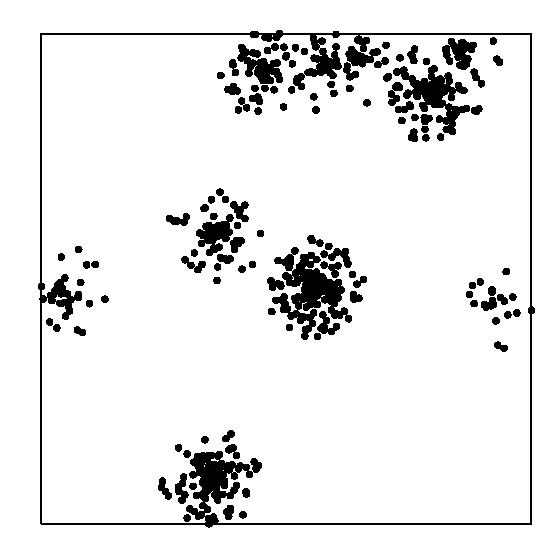
\includegraphics[scale=1]{cities1000}}
      \vbox{\hbox{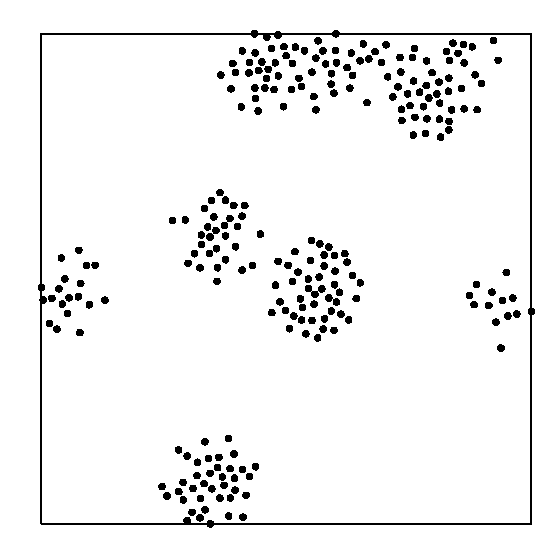
\includegraphics[scale=0.5]{dt250}}%
        \hbox{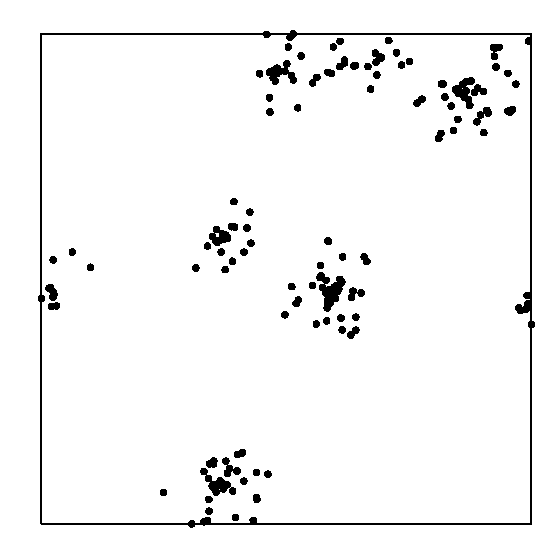
\includegraphics[scale=0.5]{cs250}}}}
  \end{center}
  \caption{Clustered 1000-point set $P$ (on the left), and two
    250-point approximations for $P$.}
  \label{fi:example_result}
\end{figure}
%%%%%%%%%%%%%%%%%%%%%%%%%%%%%%%%%%%%%%%%%%%%%%%%%%%%%%%%%%%%%%%%%
The real-world data
set represents the acres of harvested cropland in the USA in
1992~\cite{realworld}---see Fig.~\ref{fi:dotmap}.


\subsection{Computing the error}
Our heuristics call a subroutine to compute the error for given $P$
and $Q$ many times. We have implemented the $O(m^{2} n + n \log n)$
algorithm for computing the error for square ranges.  For large $n$
and $m$, this is rather slow. To speed up the heuristics we therefore
want to replace the subroutine by a faster one.  We do this by
computing the error for squares of a fixed size, for several different
sizes; for a fixed size we used the $O(n \log n)$ algorithm of
Theorem~\ref{th:unitsquares}.  The hope is that if the number of sizes
is large enough, the error we find is close enough to the real error,
so that it will not harm our heuristics. Our first experiment is to
test whether this hope is justified: we compare the real error,
computed with the $O(m^{2} n + n \log n)$ algorithm, to the error
computed by looking at squares of $k$ different sizes only, for
various values of $k$.

The results are summarized in Table~\ref{table1}.
%%
\begin{table}
{\tiny \begin{center}
\begin{tabular}{|r|c@{\hspace{3mm}}c@{\hspace{3mm}}c|c@{\hspace{3mm}}c@{\hspace{3mm}}c|c@{\hspace{3mm}}c@{\hspace{3mm}}c|c@{\hspace{3mm}}c@{\hspace{3mm}}c|c@{\hspace{3mm}}c|}\hline
& \multicolumn{6}{c|}{Uniform} & \multicolumn{6}{c|}{Clustered} & \multicolumn{2}{c|}{Real} \\ \hline
$n$ & \multicolumn{3}{c|}{1000 (20 samples)} & \multicolumn{3}{c|}{5000 (5 samples)} 
	& \multicolumn{3}{c|}{1000 (5 samples)} & \multicolumn{3}{c|}{5000 (5 samples)} & \multicolumn{2}{c|}{11000 (1set)} \\\hline
$m$ & 50 & 100 & 250 & 100 & 250 & 500 & 50 & 100 & 250 & 100 & 250 & 500 & 500 & 1000 \\ \hline
$\delta$ & 20 & 10 & 4 & 50 & 20 & 10 & 20 & 10 & 4 & 50 & 20 & 10 & 22 & 11 \\ \hline\hline
$k=5$ & 30 & 22 & 18 & 117 & 68 & 95 & 27& 22 & 18 & 160 & 88 & 82 & 68 & 10 \\
     & (104) & (80) & (80) & (296) & (183) & (401) & (121) & (74) & (92) & (517) & (230) & (307) & (68) & (10) \\ \hline
$k=10$ & 17 & 14 & 9 & 78 & 47 & 53 & 17 & 12 & 9 & 102 & 58 & 54 & 68 & 10 \\
       & (50) & (60) & (36) & (177) & (138) & (230) & (71) & (38) & (40) & (220) & (228) & (192) & (68) & (10) \\ \hline
$k=30$ & 9 & 7 & 4 & 41 & 27 & 17 & 8 & 5 & 4 & 45 & 29 & 20 & 19 & 9 \\ \hline
       & (30) & (22) & (15) & (86) & (65) & (42) & (28) & (18) & (22) & (92) & (119) & (126) & (19) & (9) \\ \hline
$k=60$ & 6 & 4 & 3 & 27 & 17 & 12 & 4 & 3 & 3 & 28 & 19 & 13 & 19 & 9 \\ \hline
       & (18) & (13) & (9) & (68) & (44) & (24) & (27) & (12) & (12) & (70) & (90) & (86) & (19) & (9) \\ \hline
\end{tabular}
\end{center}
}
\caption{Estimating the square error by $k$ fixed sizes.}
\label{table1}
\end{table}

For each distribution we have generated between 5 and 10 different
sets $P$, and for each $P$ between 8 and 20 different sets $Q$.  Half
of the choices for $Q$ were taken as random samples from $P$, the
other half was generated using another distribution.  The table shows
the average difference between the error for arbitrary squares and the
error for $k$ different fixed sizes, where the sizes were equally
spaced. (We also tried sizes on a logarithmic scale, but obtained
poorer results.) The numbers between brackets in the table give the
maximum difference found in the experiments.  If we take $k=60$, then
the average difference between the real error and the estimated error
is always close to (and often smaller than) the dot value, and the
maximum difference is close to twice the dot value.  We conclude from
this that it is safe to use the estimated error in our heuristics.

We use this estimate out of necessity.  Computing the error exactly
takes hours for the U.S.\ data set, while computing the estimated
error takes only a few seconds.  Since our algorithms for finding good
approximations have to repeatedly compute the error of an
approximation, computing the exact error is not a reasonable option.

\subsection{The heuristics}

Next, we experimented with several heuristics for generating an
approximation $Q$ of a desired size $m$ for a given set $P$ of $n$
points.  These heuristics fall into two classes:

\begin{enumerate}
\item Iterative algorithms that start with a random solution and then
apply some iteration rule to try and improve upon it. These algorithms
include traditional optimization algorithms such as simulated
annealing and taking the best of $k$ random samples.

\item Clustering algorithms that partition the set $S$ into $m$ groups
and then choose one representative point for each group.  These
algorithms may partition the point set $S$ directly (see Dobkin-Tal
below) or may partition the plane thereby inducing a partition of $S$.
\end{enumerate}

\subsubsection{Iterative algorithms}

The first class of heuristics that we consider are \emph{iterative}
algorithms.  For this class, we consider any algorithm that works by
testing many different solutions, i.e., subsets $Q$, and taking the
best one.  The differences between various iterative algorithms come
from how the subsets $Q$ are selected.

\emph{Heuristic 1: Best of $k$ random samples.}
Here we take $k$ random samples $Q_1,\ldots,Q_k$ of $P$, compute the
approximation error for each of them, and return the best sample.
Here $k$ is a parameter.  The larger the value of $k$, the better
the approximation.

\emph{Heuristic 2: Simulated annealing.}
Simulated annealing (c.f., \cite{h01}) is a general search technique
that starts with an initial random solution (i.e., a random sample)
and then tries to converge to an optimal solution by introducing
random changes.  A random change is kept if (1)~it improves the
current solution, or (2)~some \emph{annealing condition} is met.

In our implementation of simulated annealing, a random change involves
choosing a random point of $Q$ and replacing it with a random point
from $P\setminus Q$.  The annealing criterion is the following: During
the $i$th round of annealing, we replace the solution $Q$ by the
solution $Q'$ with probability $\exp((\Delta(Q,P)-\Delta(Q',P))/T_i)$.
Here, $T_i$ is a temperature parameter whose value is $T_i=(k-i)/k$,
where $k$ is the total number of rounds the algorithm runs for.


\emph{Heuristic 3: Swapping.}
We first obtain an approximation $Q$ by taking a random sample of size
$m$, and then try to improve it as follows. We compute a range
$r_{\mypos}$ with the largest positive error and a range $r_{\myneg}$
with the largest negative error.  We remove a random point in $Q \cap
r_{\myneg}$ from~$Q$, and add a random point in $(P\setminus Q) \cap
r_{\mypos}$ to~$Q$.

Initial experimental results with the swapping heuristic were
encouraging. However, this heuristic is highly dependent on having a
good starting configuration.  When this doesn't happen, the algorithm
can get stuck in a local minimum, after which no further improvement
can be made.  To overcome this problem, we implemented two variants of
the swapping heuristic.

\emph{Heuristic 4: Swapping with restart.}
This is a version of the swapping heuristic that starts with a new
random sample $Q$ if 10 consecutive rounds of swapping fail to improve
the solution.

\emph{Heuristic 5: Swapping with 10\% perturbation.}
This is a version of the swapper that, after 10 consecutive rounds of
swapping fail to improve the solution, removes $\lceil m/10\rceil$
points of $Q$ at random and replaces them with $\lceil m/10\rceil$
points of $P\setminus Q$ selected at random.

\subsection{Experimental results.} 

Fig.~\ref{fi:dotmap} shows the progress of iterative algorithms for
1000 rounds on a set $P$ of $n=5000$ points chosen uniformly at random
from the unit square.  The algorithms are attempting to find a good
approximation $Q$ of size $m=100$.  The $x$-axis of the figure
represents time (number of rounds) and the $y$-axis represents the
approximation error.  Note that, although the figure looks as if the
various heuristics began with different starting configurations, this
is cause by a lack of resolution, and is not actually the case.  All
experiments began with the same initial configuration.

\begin{figure}
\begin{center}
\begin{tabular}{c@{}c}
\raisebox{5cm}{Error} & 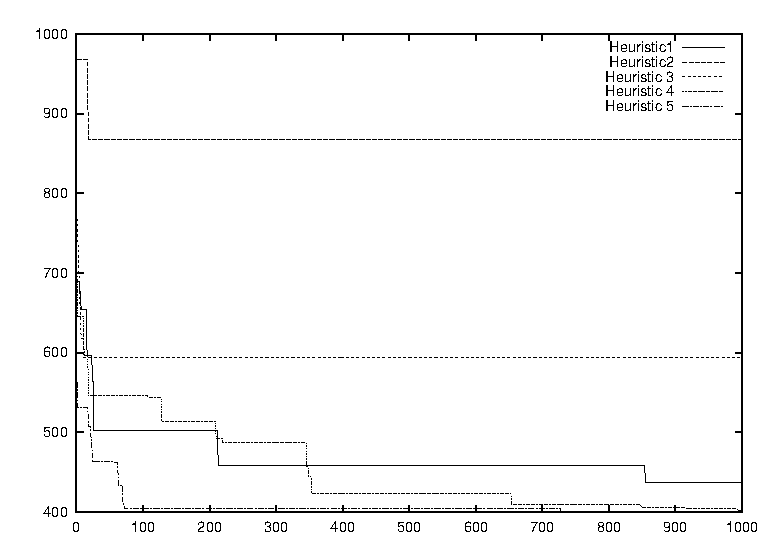
\includegraphics{iterative} \\
& Number of iterations
\end{tabular}
\end{center}
\caption{The progress of Heuristics 1-5 over 1000 rounds.}
\end{figure}

The worst of the heuristics is clearly simulated annealing
(Heuristic~2), which makes some quick improvements in the first few
rounds and then gets trapped in a local minimum.  Part of the problem
with simulated annealing is that it completely ignores the problem and
tries to make progress by introducing small random changes.  It is
very easy for the simulated annealing strategy to get stuck in a local
minimum and never improve.  Although it may be possible to improve the
performance of the simulated annealing heuristic by tweaking the
parameters, we were unable to do significantly better than the results
presented here.

The second-worst heuristic is the swapping heuristic (Heuristic 3).
The swapper performs better than simulated annealing because it
introduces a carefully-chosen change that is more likely to improve
the current solution. However, it still only changes the current
solution by one point and therefore quickly gets caught in a local
minimum.

The two best heuristics are modifications of the swapping heuristic.
Swapping with restart (Heuristic 4) and swapping with 10\%
perturbation (Heuristic 5) both achieve comparable results after 1000
rounds. However, swapping with 10\% perturbation converges more
quickly to a good solution.  This seems to be due to the fact that,
when it gets stuck in a local minimum, it restarts with a new solution
that is still much better than a random sample.

Choosing the best of $k$ random samples (Heuristic 1), a technique
that is often mentioned in the literature, does not perform as well as
the modified swapping heuristics.  It reliably finds good
approximations, but these are not quite as good as those found by the
two modified swapping heuristics.

\subsection{Clustering algorithms}

We also considered algorithms that can be loosely termed
``clustering'' algorithms.  These are algorithms that (implicitly or
explicitly) partition the point set $S$ into $m$ groups and then
select a representative point or points from each group.

\emph{Heuristic 6: Rows and columns.} This heuristic produces a
subset $Q$ with $m=r\times s$ points by first sorting the points by
$x$-coordinate and grouping the points into $r$ \emph{columns}, i.e.,
vertical strips, each containing $n/r$ points.  Next, the points
within each column are sorted and grouped into $s=m/r$ rows, i.e.,
horizontal strips, of size $n/m$.  Thus we obtain a partition of the
plane into $m$ rectangular cells each containing exactly $n/m$ points.  

For our set $Q$, we take a sample from each cell.  Several strategies
for choosing the best sample in each square were implemented.  The one
that worked best was to try $k=50$ random samples and choose the
sample with smallest error constrained to that cell.  

Note that, in these experiments, the value of $m$ is given, so we must
factor $m$ into $r$ and $s$.  We did this by taking
$r=\lfloor\sqrt{m}\rfloor$ and then taking $s$ to be the largest
integer so that $r\times s\le m$.  This gives us an approximation that
uses at most $m$ points. When computing the quality of the resulting
approximation we adjust the dot value $\delta$ accordingly. 

\emph{Heuristic 7: Quadtrees.}
This heuristic is based on the well-known quadtree data structure.
Let $S$ be some axis-aligned square containing the point set $P$.  We
recursively partition $S$ into squares as follows.  If $S$ contains
fewer than $4\delta$ points of $P$ then we do nothing.  Otherwise, we
partition $S$ into 4 equal squares and recursively partition each
square.

Once this partition is computed, we choose a sample from each square
of the partition.  If a square contains $k$ points of $P$ then we
choose a sample of size $\lfloor k/\delta+1/2\rfloor$ from that
particular square.  The sampling strategy is the same used for
Heuristic~6.  As before, this does not always yield a solution with
exactly $n/\delta$ points so, when computing the error we adjust the
dot value $\delta$ accordingly.


\emph{Heuristic 8: Dobkin-Tal.}
The algorithm proposed by Dobkin and Tal~\cite{dt-esrla-01} produces
an approximation that is not a subset of $P$, by repeatedly finding
closest pairs and replacing them by their midpoint.

Dobkin and Tal were originally interested in the dual setting of our
problem: given a set of lines, find a smaller set of lines whose
arrangement approximates the original arrangement.  They solve the
problem using dualization, so they arrive exactly at our
problem. 

Although their approach seems more suited to minimizing the Hausdorff
distance between $P$ and $Q$---indeed, they prove bounds on the
minimal Hausdorff distance they achieve---they also use their
algorithm in an application that is closely related to ours.  Namely,
they want to approximate the area half-plane discrepancy~\cite{c01} of
$P$ with the discrepancy of $Q$. (The area half-plane discrepancy of a
set of points in the unit square is defined as the maximum, over all
half-planes, of the absolute difference between the fraction of points
in the half-plane and the fraction of the unit square covered by the
half-plane.)  Now if we considered half-planes as regions, then the
approximation error of $Q$ with respect to $P$ is an upper bound on
the difference between the area discrepancies of $P$ and $Q$.  Dobkin
and Tal claim that for some distributions of $P$ the area discrepancy
of $P$ can be estimated better by a set $Q$ computed with their
algorithm than by a random sample. For this reason we also consider
their algorithm in our experiments.

\subsection{Experimental results.}

Table~\ref{tab:results} shows the results for Heuristic~5, the best of
the iterative heuristics, after 50 rounds and all the clustering
algorithms.  The tests were performed on 6 data sets of size $n=5000$
and one real world data set.  The data sets U5K\{a,b,c\} each consist
of 5000 points uniformly distributed in the unit square.  The data
sets C5K\{a,b,c\} each consist of 5000 points drawn from the ``city''
distribution described earlier.  The US1 data set is the data set
shown in Fig.~\ref{fi:dotmap} and consists of 82516 points.  For each
data set, we used the algorithms to compute approximations with dot
values $\delta=100,50,20$ and 10.

 
\begin{table}
\begin{center}\begin{tabular}{|r|r|r|rrr|rrr|}\hline\hline
Heuristic  & $\delta$ 
                 &  US1 & U5Ka & U5Kb & U5Kc & C5Ka & C5Kb & C5Kc\\\hline 
           & 100 & 3206 &  570 &  674 &  655 &  570 &  730 &  680 \\
Heuristic 5&  50 & 3066 &  556 &  507 &  427 &  515 &  407 &  614 \\
(Swap w. 10\%)&20&4396& 359 &  268 &  310 &  364 &  368 &  343 \\ 
           &  10 &  789 &  309 &  236 &  243 &  227 &  231 &  223 \\\hline
           & 100 & 1924 &  650 &  682 &  657 &  491 &  487 &  524 \\
Heuristic 6&  50 & 1036 &  705 &  359 &  748 &  405 &  410 &  367 \\
(Rows \& Cols.)&20&885 &  315 &  256 &  294 &  188 &  273 &  203 \\
           &  10 &  780 &  153 &  195 &  156 &  119 &  128 &  132 \\\hline
           & 100 & 2289 &  582 &  604 &  739 &  520 &  400 &  524 \\
Heuristic 7&  50 & 1612 &  500 &  508 &  356 &  421 &  321 &  353 \\
(Quadtree) &  20 & 4285 &  261 &  230 &  276 &  225 &  217 &  207 \\
           &  10 & 6728 &  439 &  467 &  398 &  398 &  396 &  343 \\\hline
           &  100&  --- &  824 &  742 &  691 & 1445 & 1806 & 1335 \\
Heuristic 8&  50 &  --- &  575 &  519 &  704 & 1479 & 1752 & 1133 \\
(Dobkin-Tal)& 20 &  --- &  414 &  392 &  399 & 1378 & 1631 & 1028 \\
           &  10 &  --- &  280 &  302 &  309 & 1302 & 1586 & 1011 \\ \hline
\end{tabular}\end{center}
\caption{Experimental results for clustering algorithms.}
\label{tab:results}
\end{table}

These results suggest that the ``rows and columns'' heuristic seems to
be the best choice of the clustering heuristics.  For large values of
$\delta$, it is competitive with the quadtree heuristic and much
better than Dobkin-Tal.  For small values of $\delta$, the ``rows and
columns'' heuristic is definitely the method of choice and outperforms
the quadtree heuristic by a significant margin.  This seems to be
because the quadtree heuristic has trouble controling the number of
points in each cell, while the ``rows and columns'' heuristic has
exactly $\delta$ points per cell.

Surprisingly, the simple ``rows and columns'' heuristic also seems to
perform better than Heuristic~5, even though we allow Heuristic~5 to
run for 50 rounds.  This makes the ``rows and columns'' heuristic a
very fast method of obtaining good quality solutions.  In terms of
computation time, the entire running time of the rows and columns
heuristic is roughly the same as one or two rounds of an iterative
heuristic.

Finally, the Dobkin-Tal heuristic does reasonably well for uniformly
distributed points, but does very poorly with clustered point
sets. This seems to be an artifact of the averaging effect obtained by
repeatedly taking the midpoints of the pairs of points.

% \noindent\emph{Other heuristics.}
% We also tried heuristics that construct an approximation
% incrementally. Suppose we have already constructed an approximation
% $Q_i$ consisting of $i$ points. Then we create the approximation
% $Q_{i+1}$ by choosing $k$ points at random from $P\setminus Q_i$,
% evaluate the error in $Q_i \cup \{q\}$ for each chosen point $q$, and
% add the best $q$ to $Q_i$ to obtain $Q_{i+1}$.  In another approach,
% we first obtain a random sample that is too large (say, of $2m$
% points), and then iteratively remove a random point in a range with
% the largest negative error.  However, neither approach leads to
% satisfactory results.  \medskip


%%%%%%%%%%%%%%%%%%%%%%%%%%%%%%%%%%%%%%%%%%%%%%%%%%%%%%%%%%%%%%%%%%%
\section{Concluding remarks}
\label{se:concl}
%%%%%%%%%%%%%%%%%%%%%%%%%%%%%%%%%%%%%%%%%%%%%%%%%%%%%%%%%%%%%%%%%%%
In some applications, it may be desirable to give outliers in $P$ a
bigger chance to be present in $Q$.  This can be done by giving these
points a higher weight. For instance, we can let the weight of each
point be dependent on the number of points within a fixed distance
from that point. By giving more and more weight to isolated points,
the approximation is likely to become more and more uniform.  The
definition of approximation error and our algorithms can easily be
extended to the weighted case, and it would be interesting to
experiment with this.  

In our application it seems most reasonable to look at the
approximation error for families of squares or discs.  We studied the
case of squares, but it would be interesting to see if our algorithm
to compute the approximation error in this case can be improved.  We
did not study discs at all in this paper.  It is easy to compute the
approximation error for discs in (close to) cubic time, but it remains
open whether this can be done faster.

Finally, we suspect that computing the best approximation of a given
size with respect to a given set $P$ is NP-hard, but we have not been
able to prove this.

%\newpage
%%%%%%%%%%%%%%%%%%%%%%%%%%%%%%%%%%%%%%%%%%%%%%%%%%%%%%%%%%%%%%%%%%%
\bibliographystyle{plain}

\begin{thebibliography}{99}
\frenchspacing

\bibitem{a-rs-97}
  P.K.~Agarwal.
  Range searching. In: J.E.~Goodman and R.~Pollack.
  \newblock{\em Handbook of Discrete and Computational Geometry}.
  \newblock CRC Press, 1997, pages 575--598.
  
\bibitem{bg-isda-95}
  T.C.~Bailey and A.C.~Gatrell.
  \newblock{\em Interactive Spatial Data Analysis}.
  \newblock Longman Scientific \& Technical, 1995.

%%% \bibitem{b-ppadt-84}
%%%   J. Bentley.
%%%   \newblock{Programming Pearls: Algorithm Design Techniques}
%%%   \newblock{\em Communications of the ACM}, 27(9), p. 865--871, 1984.

\bibitem{bkos-cgaa-97}
  M.~de~Berg, M.~van Kreveld, M.~Overmars, and O.~Schwarzkopf.
  \newblock {\em Computational Geometry: Algorithms and Applications}.
  \newblock Springer-Verlag, Berlin, 1997.

\bibitem{bkmmm-trgps-01}
  P. Bose, M. van Kreveld, A. Maheshwari, P. Morin and J. Morrison.
  \newblock{Translating a regular grid over a point set.}
  \newblock{\em Computational Geometry: Theory and Applications},
  25:21--34, 2003. 
  
\bibitem{c01}
  B. Chazelle.
  \newblock \emph{The Discrepancy Method: Randomness and Complexity.}
  \newblock Cambridge University Press, 2000.

\bibitem{d-ctmd-99}
  B.D.~Dent.
  \newblock {\em Cartography: Thematic Map Design}.
  \newblock WCB McGraw-Hill, 1999.

%%%  \bibitem{dl01}
%%%  L. Devroye and G. Lugosi.
%%%  \newblock {\em Combinatorial Methods in Density Estimation}
%%%  \newblock Springer-Verlag, 2001.

\bibitem{dem96}
D. Dobkin, D. Eppstein, and D. Mitchell.
\newblock Computing the Discrepancy with Applications to Supersampling Patterns.
\newblock {\em ACM Transactions on Graphics}, 15:354--376, 1996.

\bibitem{dg95}
D. Dobkin and D. Gunopulos.
\newblock Concept Learning with Geometric Hypotheses.
\newblock in {\em Proc. Conf. on Comp. Learning Theory}, pages 329--344, 1995.

\bibitem{dgm96}
D. Dobkin, D. Gunopulos, and W. Maass.
\newblock Computing the Maximum Bichromatic Discrepancy with applications in Computer Graphics and Machine Learning.
\newblock {\em Journal of Computer and Systems Sciences}, 52(3):453--470, 1996.


\bibitem{dt-esrla-01}
  D.P.~Dobkin and A.~Tal.
  \newblock Efficient and small representations of line arrangements
  with applications.
  \newblock In {\em Proc. 17th Annu. ACM Sympos. Comput. Geom.},
  pages 293--301, 2001.

\bibitem{ditz}
  R.~Ditz. The visualization of population distribution in a carthographic
  information system---Aspects of technical realization of dot maps on screen.

\bibitem{gk00}
P. Goldberg and S. Kwek.
\newblock Precision of Query Points as a Resource for Learning Convex Polytopes
with Membership Queries.
\newblock In {\em Proc. Conf. on Comp. Learning Theory}, pages 225--235, 2000.

\bibitem{h01} 
J. Hromkovic. 
\newblock \emph{Algorithmics for hard problems.}
\newblock Springer-Verlag, 2001.

%%%  \bibitem{o01}
%%%  V. Ostromoukhov.
%%%  \newblock A simple and Efficient Error-Diffusion Algorithm.
%%%  \newblock In {\em Proc. of SIGGRAPH}, pages 567--572, 2001.

\bibitem{oy-nubkm-91}
  M.H.~Overmars and C.K.~Yap.
  \newblock New upper bounds in Klee's Measure Problem.
  \newblock {\em SIAM J. Comput.} 20:1034--1045 (1991).

\bibitem{realworld}
  Resource Assesment Division.
  Natural Resources Conservation Service -- USDA.
  Acres of harvested cropland, 1992.
  \url{http://www.nhq.nrcs.usda.gov/land/meta/m2815.html}

\bibitem{s-dqmsd-91}
P.~Shirley.
\newblock Discrepancy as a quality measure for sample distributions.
\newblock In F.~H. Post and W.~Barth, editors, {\em Proc. Eurographics'91},
  pages 183--194, Vienna, Austria, September 1991. Elsevier Science.

%%%  \bibitem{u88}
%%%  R. Ulichney.
%%%  \newblock Dithering with Blue Noise.
%%%  \newblock {\em Proceedings of the IEEE}, 76(1):56--79, 1988.

\bibitem{vc71} V. N. Vapnik and A. J. Chervonenkis.
  \newblock On the uniform convergence of relative frequencies of events
  to their probabilities.
  \newblock {\em Theory of Probability and Its Applications.}
  16:264--280 (1971).


\end{thebibliography}

\patscomment{
Table~\ref{table2} shows our results.  All errors
were computed using squares of 60 fixed sizes.  Each column was
computed for only one set $P$. \comment{Perhaps we should repeat the
  generate at least a few sets for each distribution ?}
%
\begin{table}
  \input{table2.tex}
  \caption{Various heuristics.
    \label{table2}}
\end{table}
\medskip
}

%%%%%%%%%%%%%%%%%%%%%%%%%%%%%%%%%%%%%%%%%%%%%%%%%%%%%%%%%%%%%%%%%%%

\end{document}
